\chapter{Practical analyses and experiments on a simulations and datasets}
\label{chap:02}
\setlength{\parskip}{1em}

\section{Simulations of supply chain attacks and related security processes}
\subsection{Initial setup and specifics simulation iterations}
From a practical standpoint, the proposed approaches can already be integrated into existing systems. For this purpose, we prepared a case study based on the PyPI software repository, which hosts multiple Python packages and operates under a FOSS (Free and Open Source Software) model. Under this model, policies allow any user to use the package manager or other mechanisms to upload, download, and publish packages in the form of source or build distributions. Our methodology is intended to enhance SCA and to establish the principle of a continuous security lifecycle, in which containment is applied prior to publication or modification, rather than immediately accepting changes into the public repository, as illustrated in Figure \ref{fig:secure_software_pipeline}. Figure \ref{fig:overview_of_software_analysis_process_in_dfd_part_1} shows the internal process of the analysis platform in a data-flow diagram. Other details of the analysis system and its engine are shown in Figure \ref{fig:overview_of_software_analysis_process_part_2_with_analysis_engine}.

\begin{figure}[htbp]
    \centering
    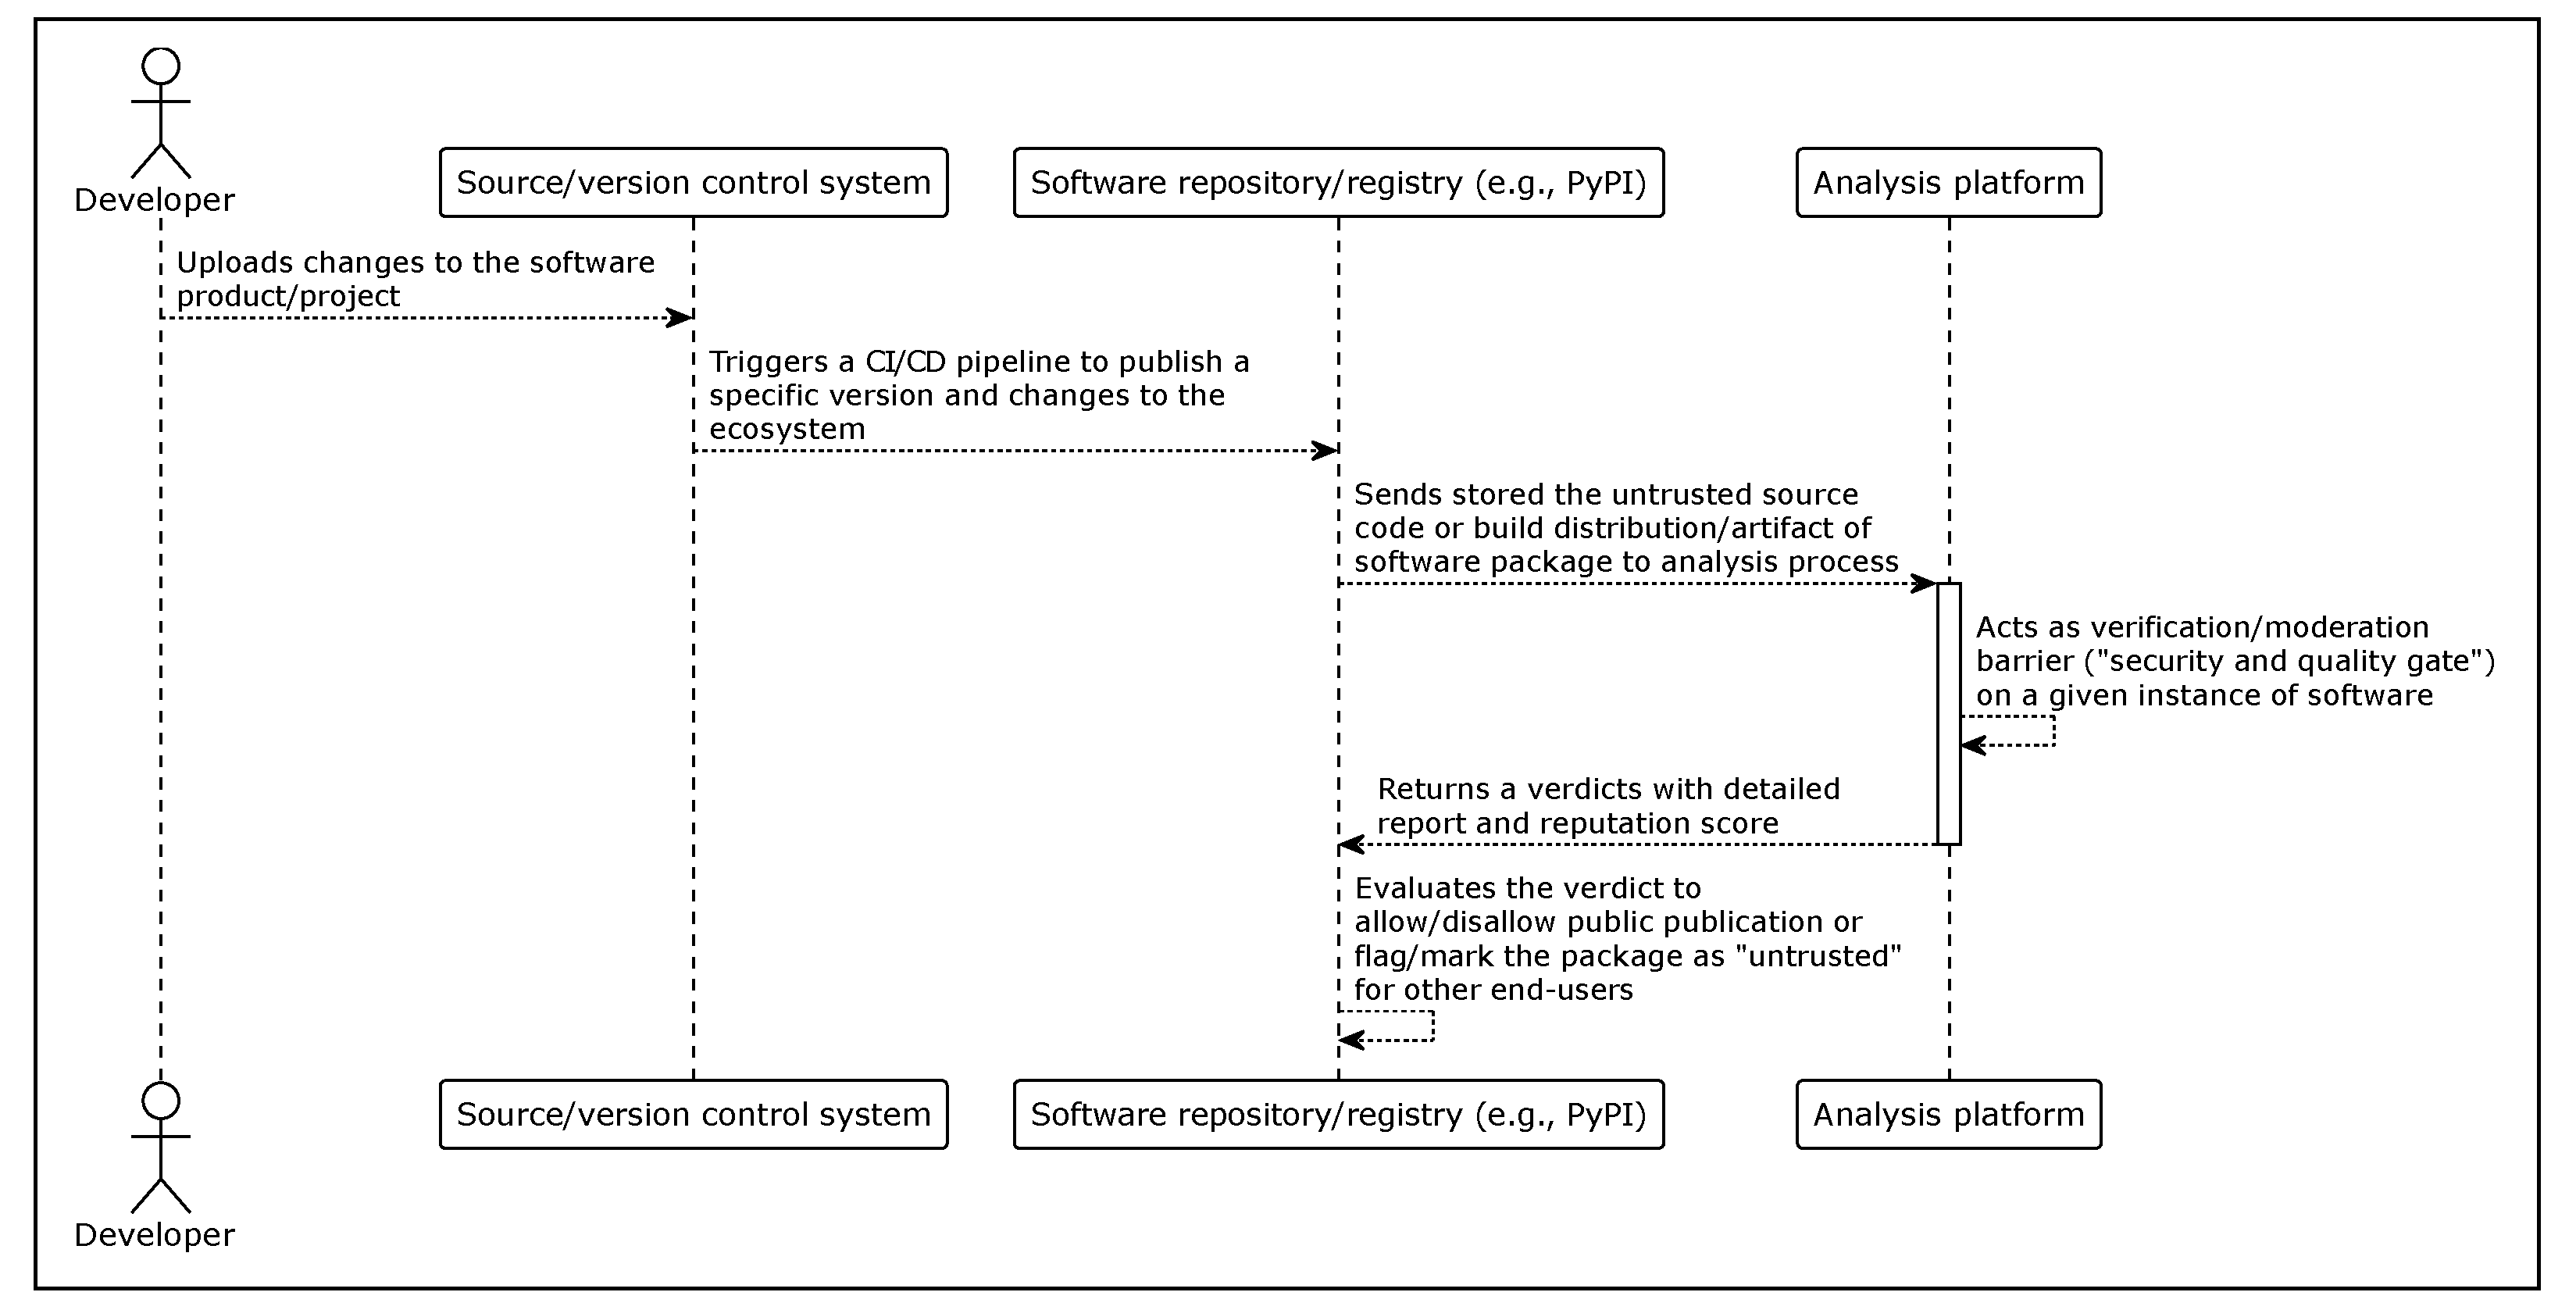
\includegraphics[width=1.0\textwidth]{../figures/secure_software_pipeline.pdf}
    \caption{Secure software pipeline by integrating the proposed analysis platform (Part 1 of PyPI example).}
    \label{fig:secure_software_pipeline}
\end{figure}

\begin{figure}[htbp]
    \centering
    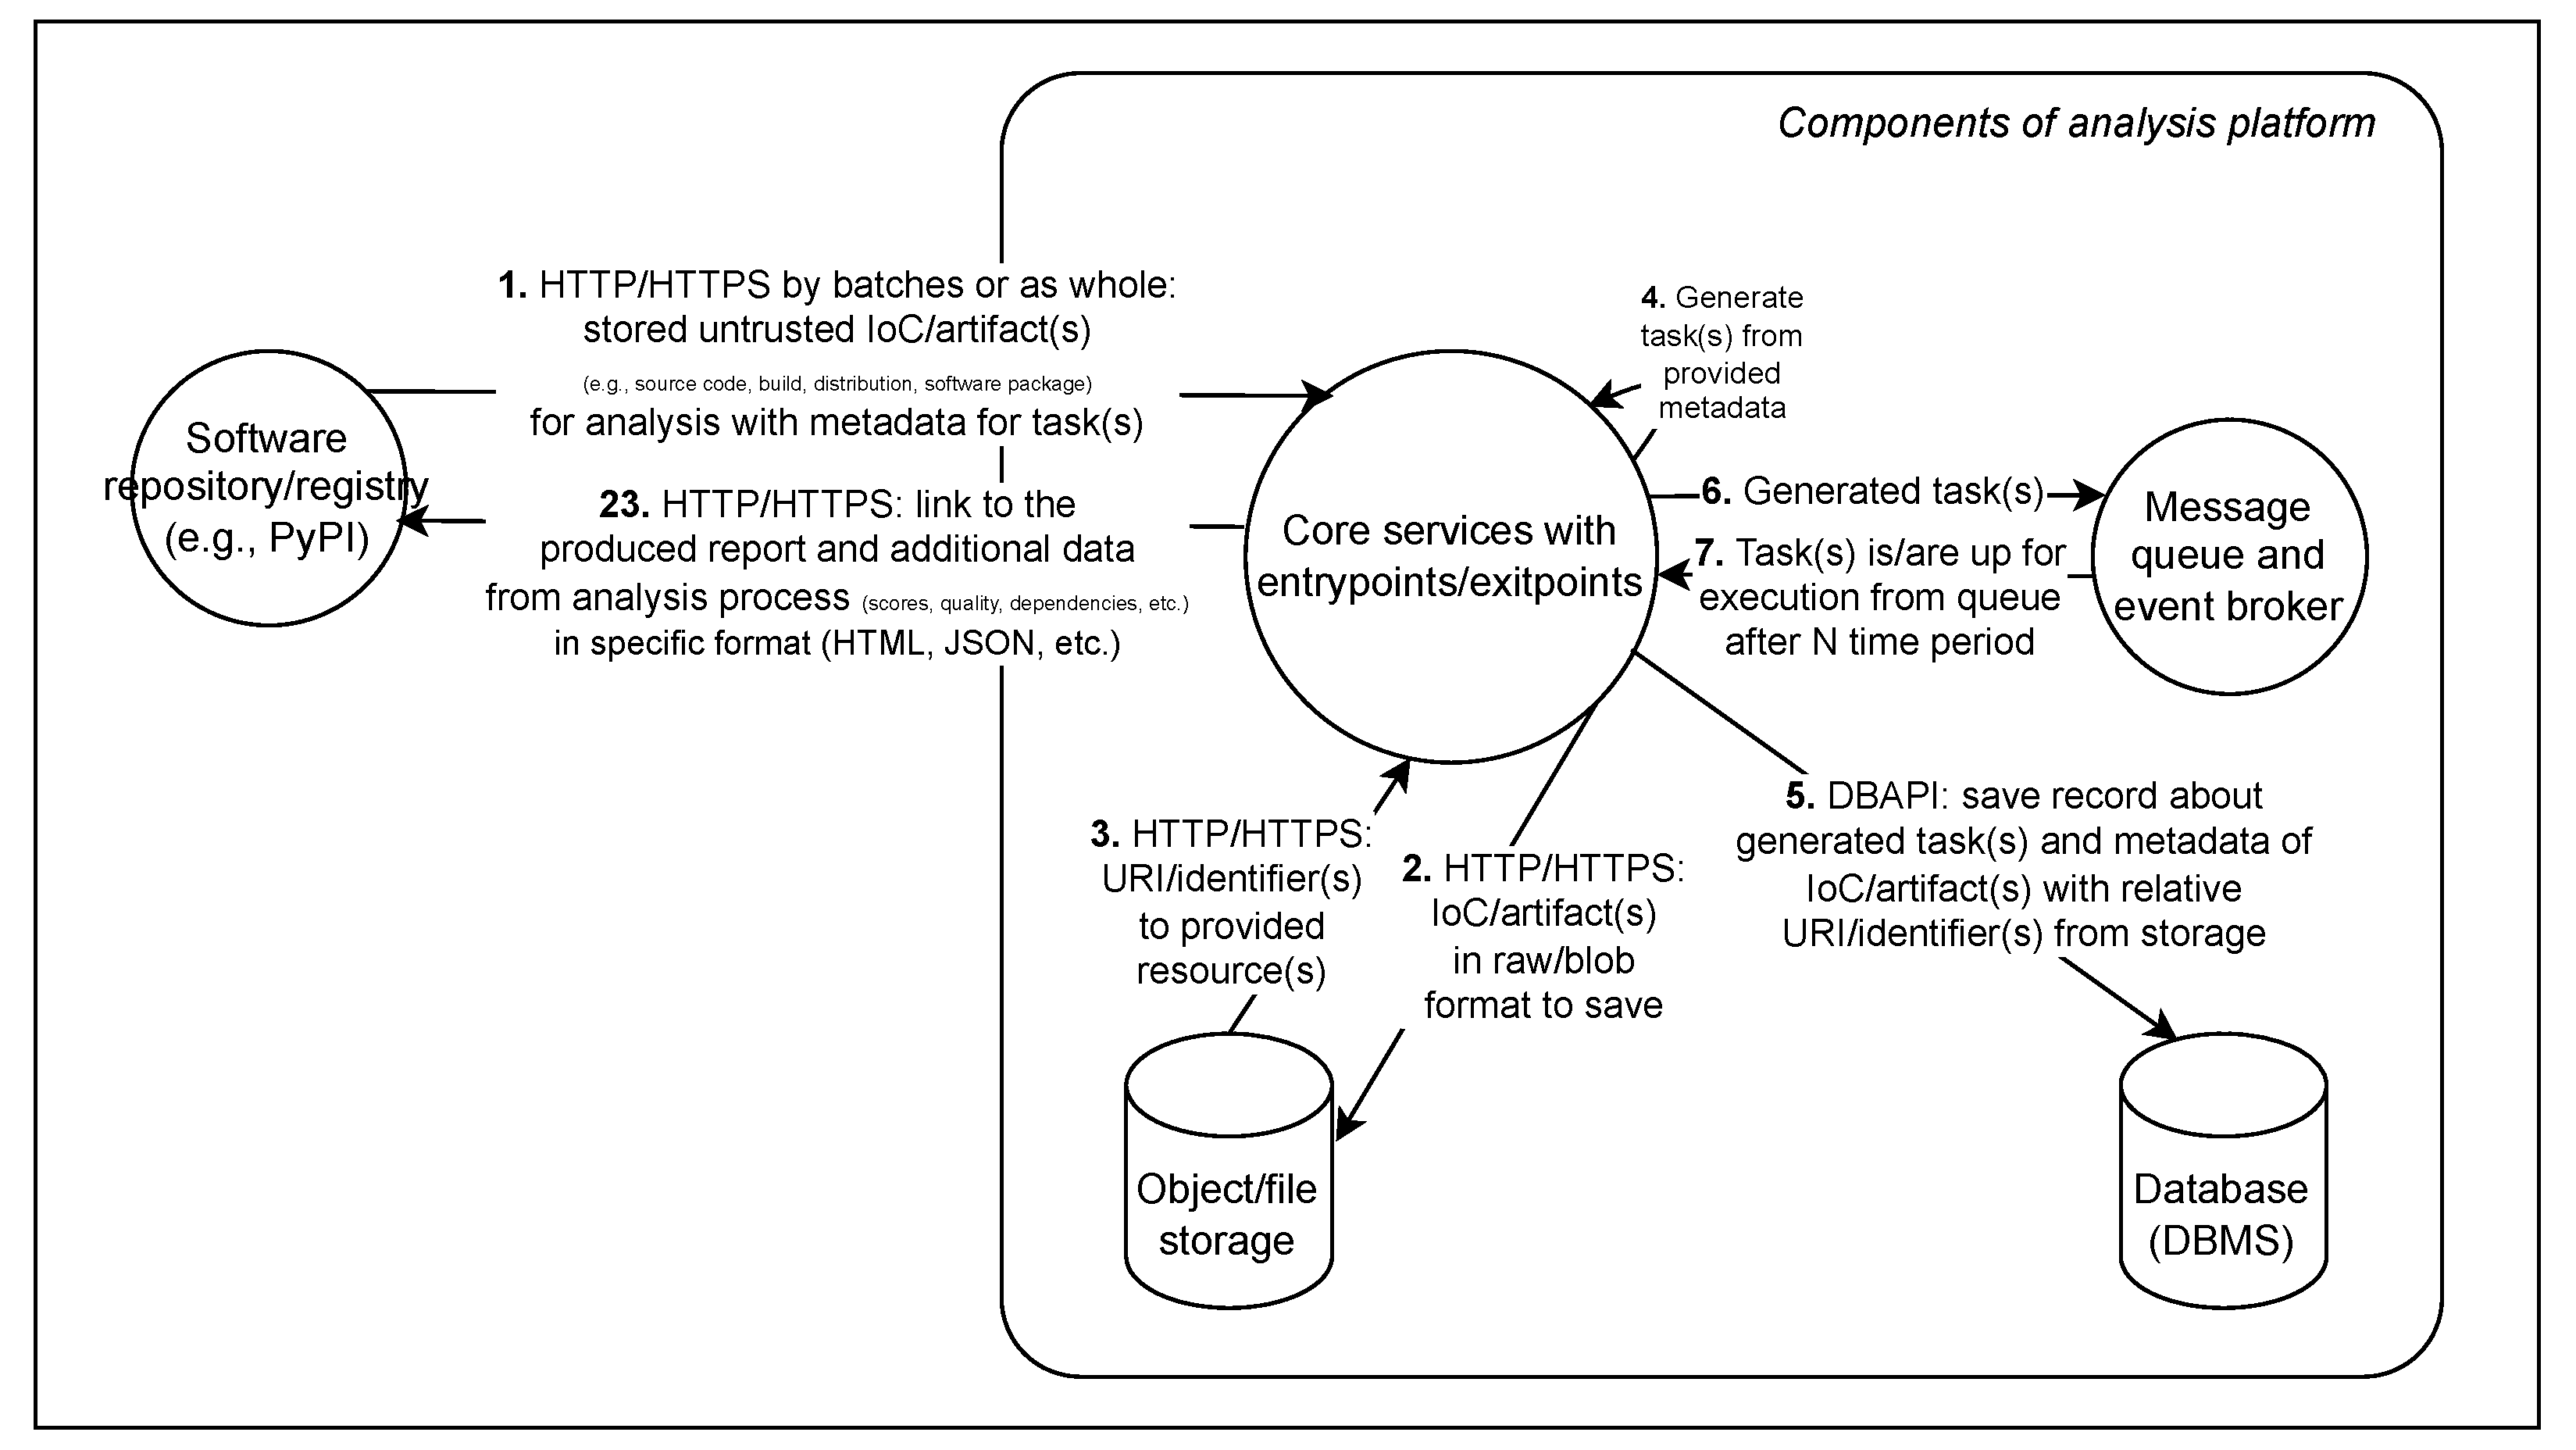
\includegraphics[width=1.0\textwidth]{../figures/overview_of_software_analysis_process_in_dfd_part_1.pdf}
    \caption{Internal processes of the analysis platform in data-flow diagram (Part 2 of PyPI example).}
    \label{fig:overview_of_software_analysis_process_in_dfd_part_1}
\end{figure}

\begin{figure}[htbp]
    \centering
    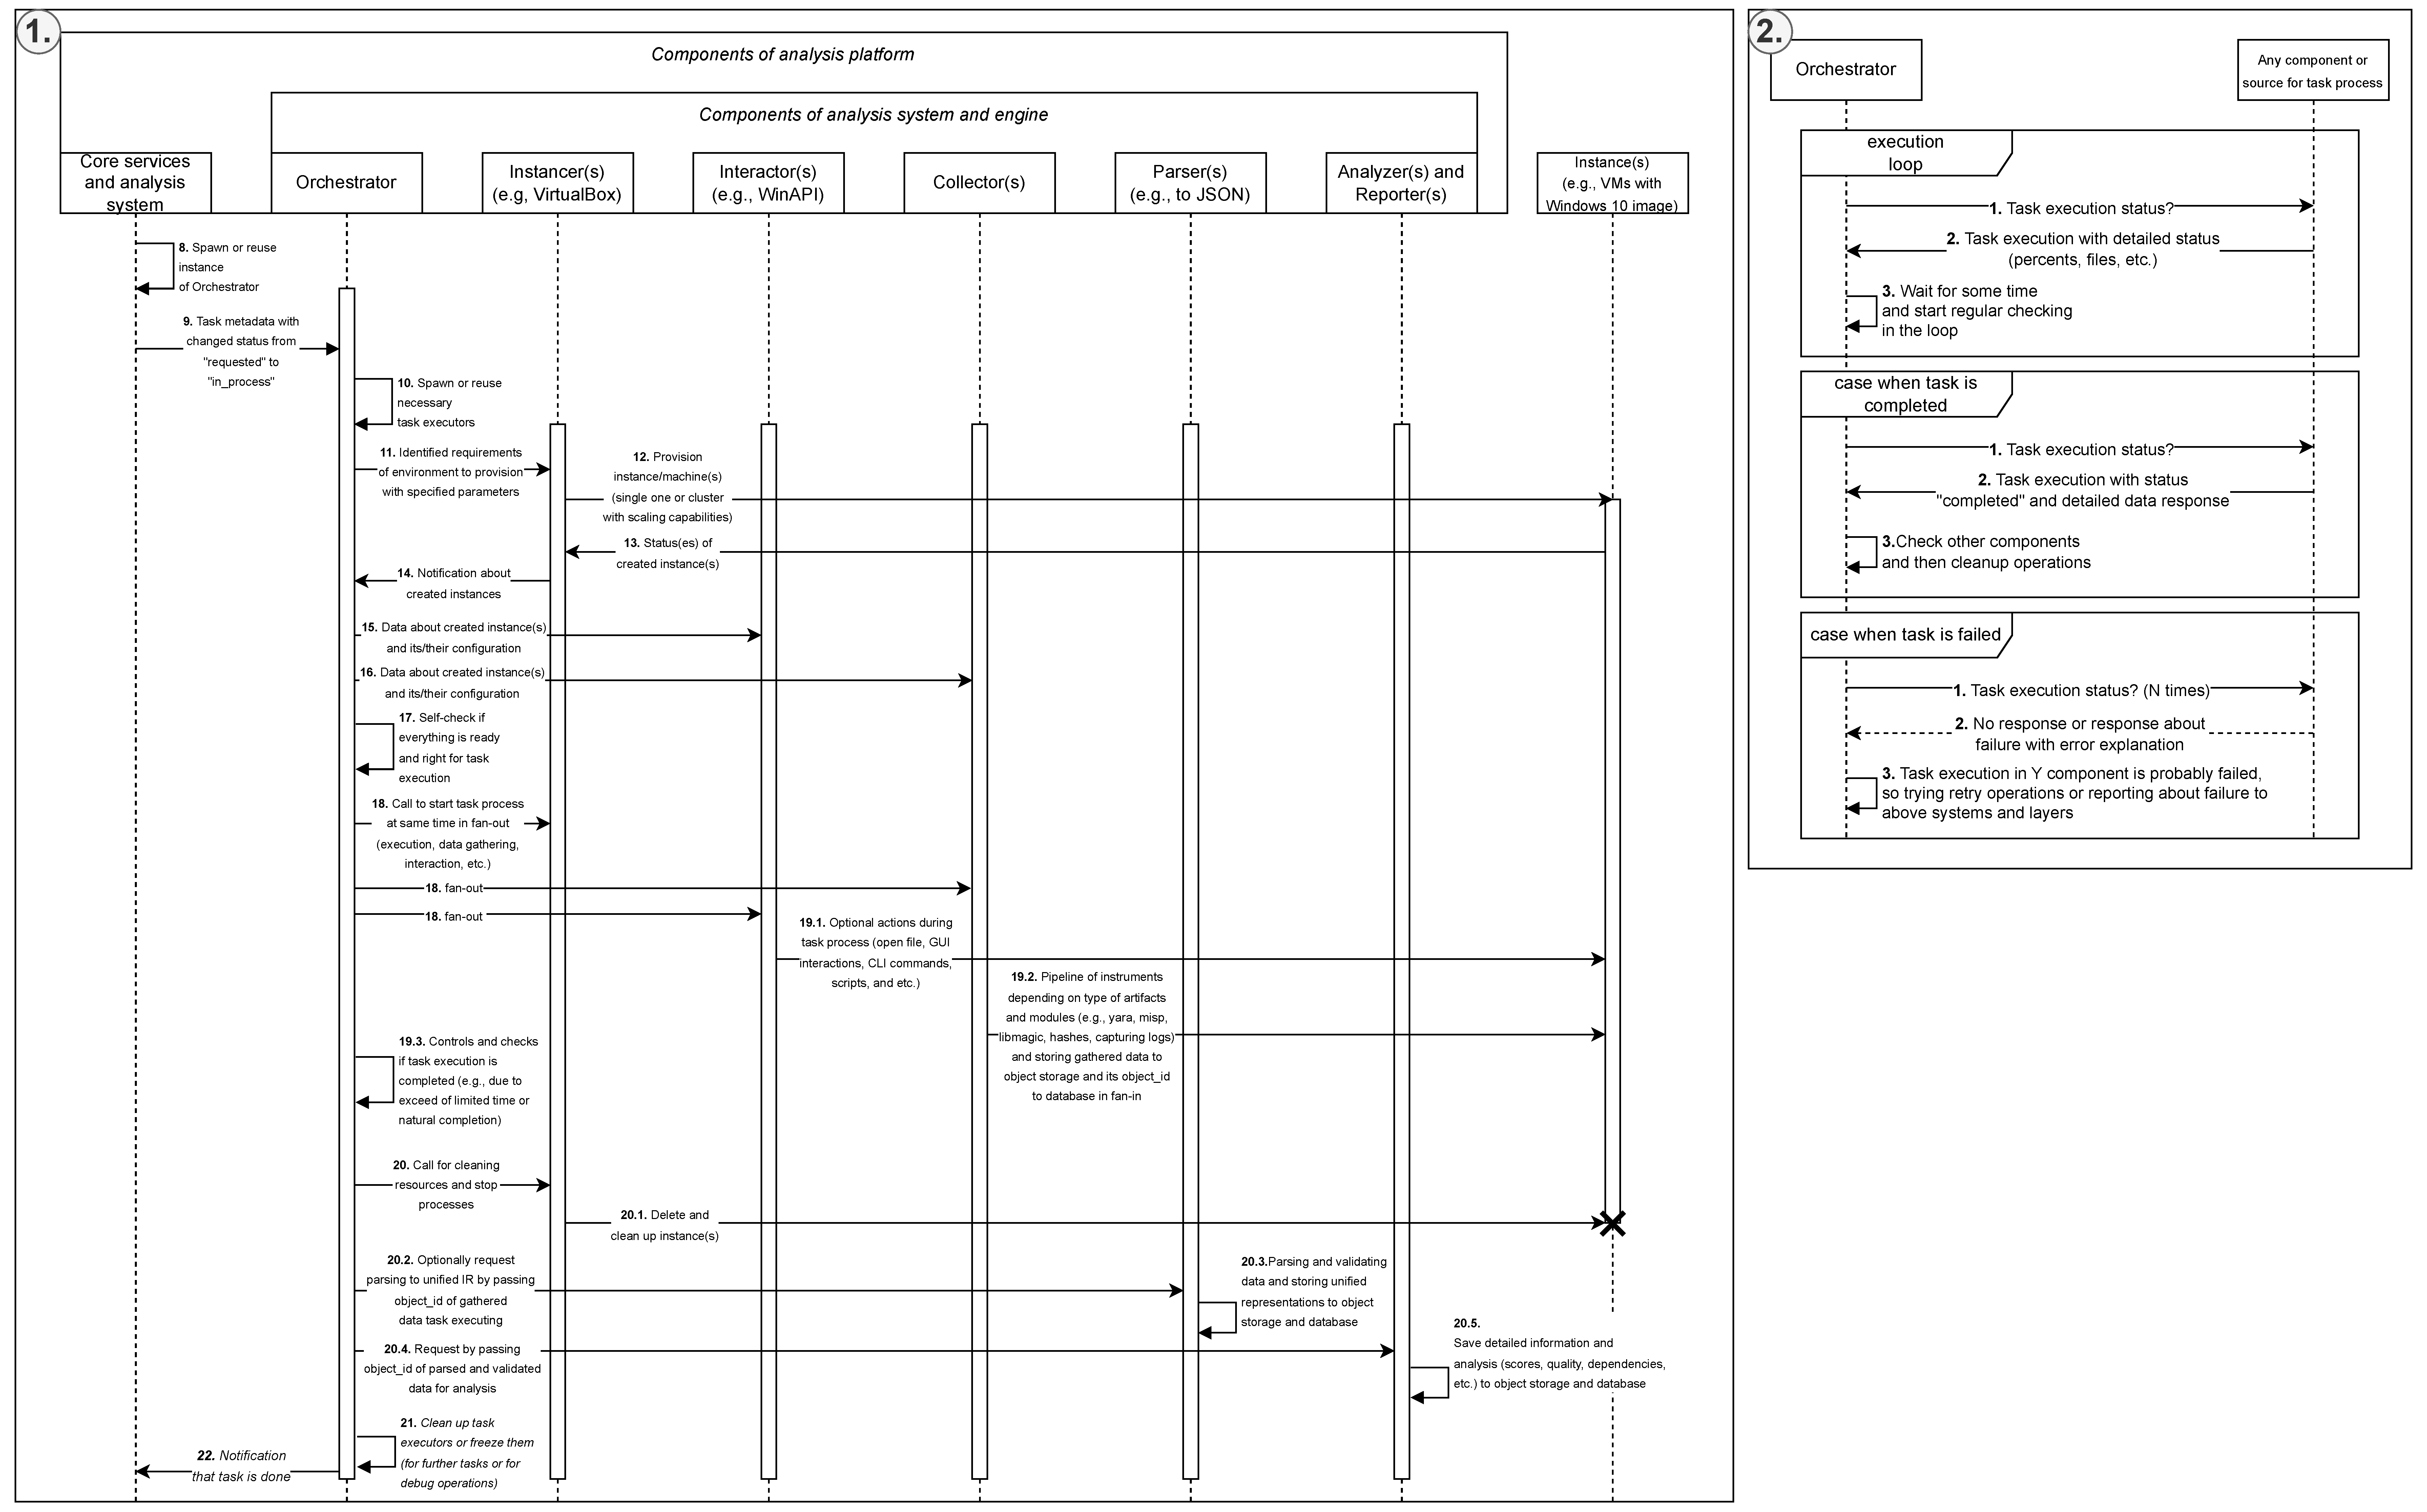
\includegraphics[width=1.0\textwidth]{../figures/overview_of_software_analysis_process_part_2_with_analysis_engine.pdf}
    \caption{Internal processes of the analysis system and its engine in a sequence diagram (Part 3 of PyPI example).}
    \label{fig:overview_of_software_analysis_process_part_2_with_analysis_engine}
\end{figure}

\newpage

Therefore, we developed a closed-system computer simulation designed to analyze various dynamics, trends, and potential practical outcomes within a software supply chain. Our primary objective is to conduct a comparative analysis between a reactive approach and a preventive security setup based on a variety of systemic factors. Firstly, we utilized the SimPy library in Python for developing discrete event simulations with defined specific actors and programmed their individual behaviors to accurately model real-world interactions within the repository at a regular rate \cite{tendikov2026aitu}. Secondly, each simulation step represents one day, with actors performing one action per step. Thirdly, each actor's progression is defined by a specific set of actions, each with a customizable probability of occurrence:
\begin{itemize}
    \item Developer (i.e., regular user) can install packages with specific version specifiers, manage existing installations, and report suspicious packages to the repository. Additionally, users can perform self- checks to detect potential compromises caused by malicious packages. This detection occurs after a 1-7 day delay, after which the developer has a 50\% chance to successfully remediate the compromise and restore their status.
    \item Package publisher can create new packages and release updated versions within the repository. However, these actions are governed by specific repository constraints, including limits on the number of packages per publisher, total upload volumes, and restrictions on the maximum number of versions allowed.
    \item Threat actor can release new versions of packages by impersonating and taking control over legitimate publishers, simulating a hijacked account. This allows them to compromise dependencies or launch supply chain attacks designed to infect regular users.
\end{itemize}

\subsection{Analysis of simulation results}

The practical results of the simulation iteration are presented below, alongside specific parameters detailed in Table \ref{tab:parameters_of_the_simulation_iteration}.

\begin{table}[htbp]
    \centering
    \begin{tabular}{|l|p{6cm}|}
        \hline
        \textbf{Fields} & \textbf{Values} \\
        \hline
        random\_seed & 42 \\
        \hline
        num\_developers & 300 \\
        \hline
        num\_threat\_actors & 5 \\
        \hline
        num\_publishers & 30 \\
        \hline
        max\_packages & 500 (unique by names) \\
        \hline
        max\_packages\_per\_publisher & 20 \\
        \hline
        max\_package\_versions & 9 (variation of package) \\
        \hline
        max\_steps & 365 \\
        \hline
        developer\_actions & check\_state: 45\%, install\_package: 20\%, change\_package: 30\%, remove\_package: 5\% \\
        \hline
        publish\_actions & publish\_package: 25\%, update\_package: 75\% \\
        \hline
        developer\_decompromise\_success & 50\% \\
        \hline
        package\_compromisation\_reveal\_time & range(7, 14) \\
        \hline
        threat\_actor\_attack\_rate & 14 \\
        \hline
    \end{tabular}
    \caption{Parameters of the simulation iteration}
    \label{tab:parameters_of_the_simulation_iteration}
\end{table}

Figures \ref{fig:compromisation_trends_in_simulation} and \ref{fig:integrity_snapshot_in_simulation} illustrate the propagation of compromised packages compared to clean packages and the final state of the simulation iteration. Firstly, the simulation shows a rapid creation of clean packages because package publishers perform actions at every step. We acknowledge that this is a limitation of our model, as real-world publishers release new versions or separate packages much less frequently. Secondly, the results for both package types eventually reach a plateau because the model enforces strict limits on the number of versions per package, the number of packages per publisher, and the total number of packages in the ecosystem. If these constraints were removed, the growth would likely follow an exponential trajectory. Despite these limits, the data on figures shows that the number of compromised developers fluctuates around 100 out of a total of 300 developers. This indicates that even a small count of 261 infected package instances out of 2476 total packages can affect one-third of all developers, according to our model. Thirdly, the outcomes are also heavily influenced by the predefined "developer\_actions" parameters. In a real- world setting, developers do not check their status as consistently as the model suggests, but instead primarily interact with the ecosystem by uploading packages for specific tasks at irregular intervals.

\begin{figure}[htbp]
    \centering
    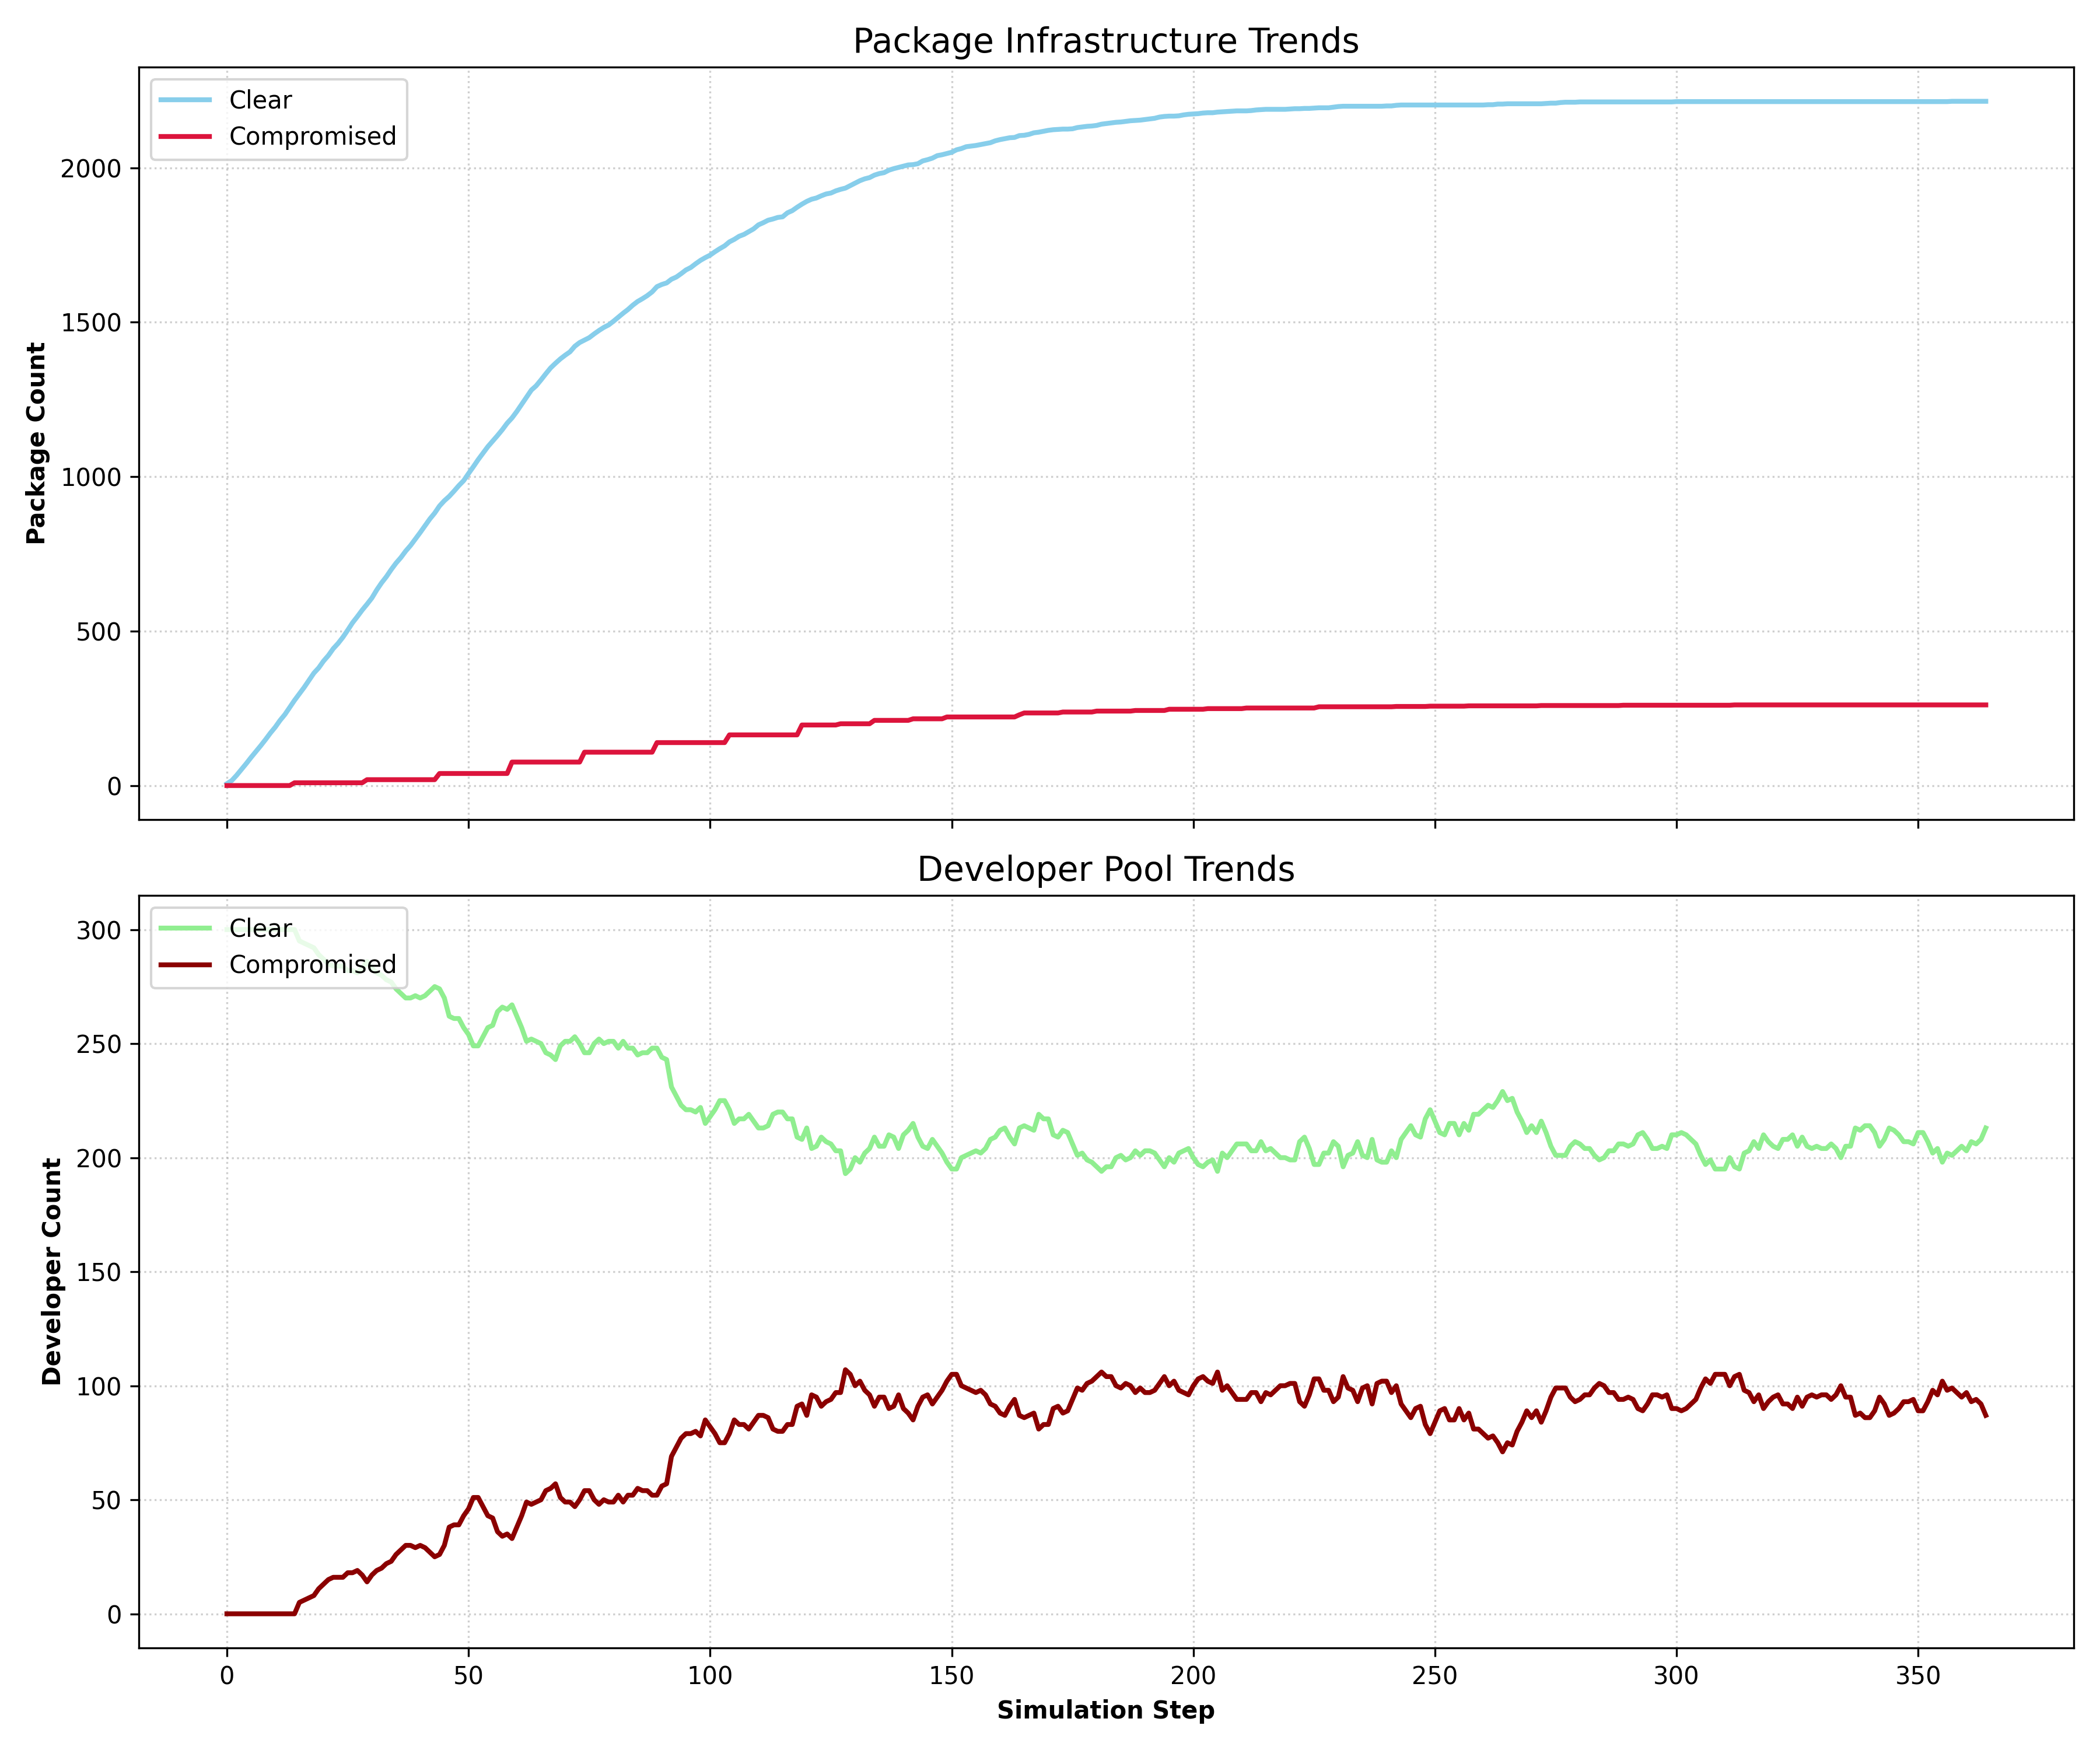
\includegraphics[width=1.0\textwidth]{../figures/compromisation_trends_in_simulation.png}
    \caption{Trends in compromises of package and developer.}
    \label{fig:compromisation_trends_in_simulation}
\end{figure}

\begin{figure}[htbp]
    \centering
    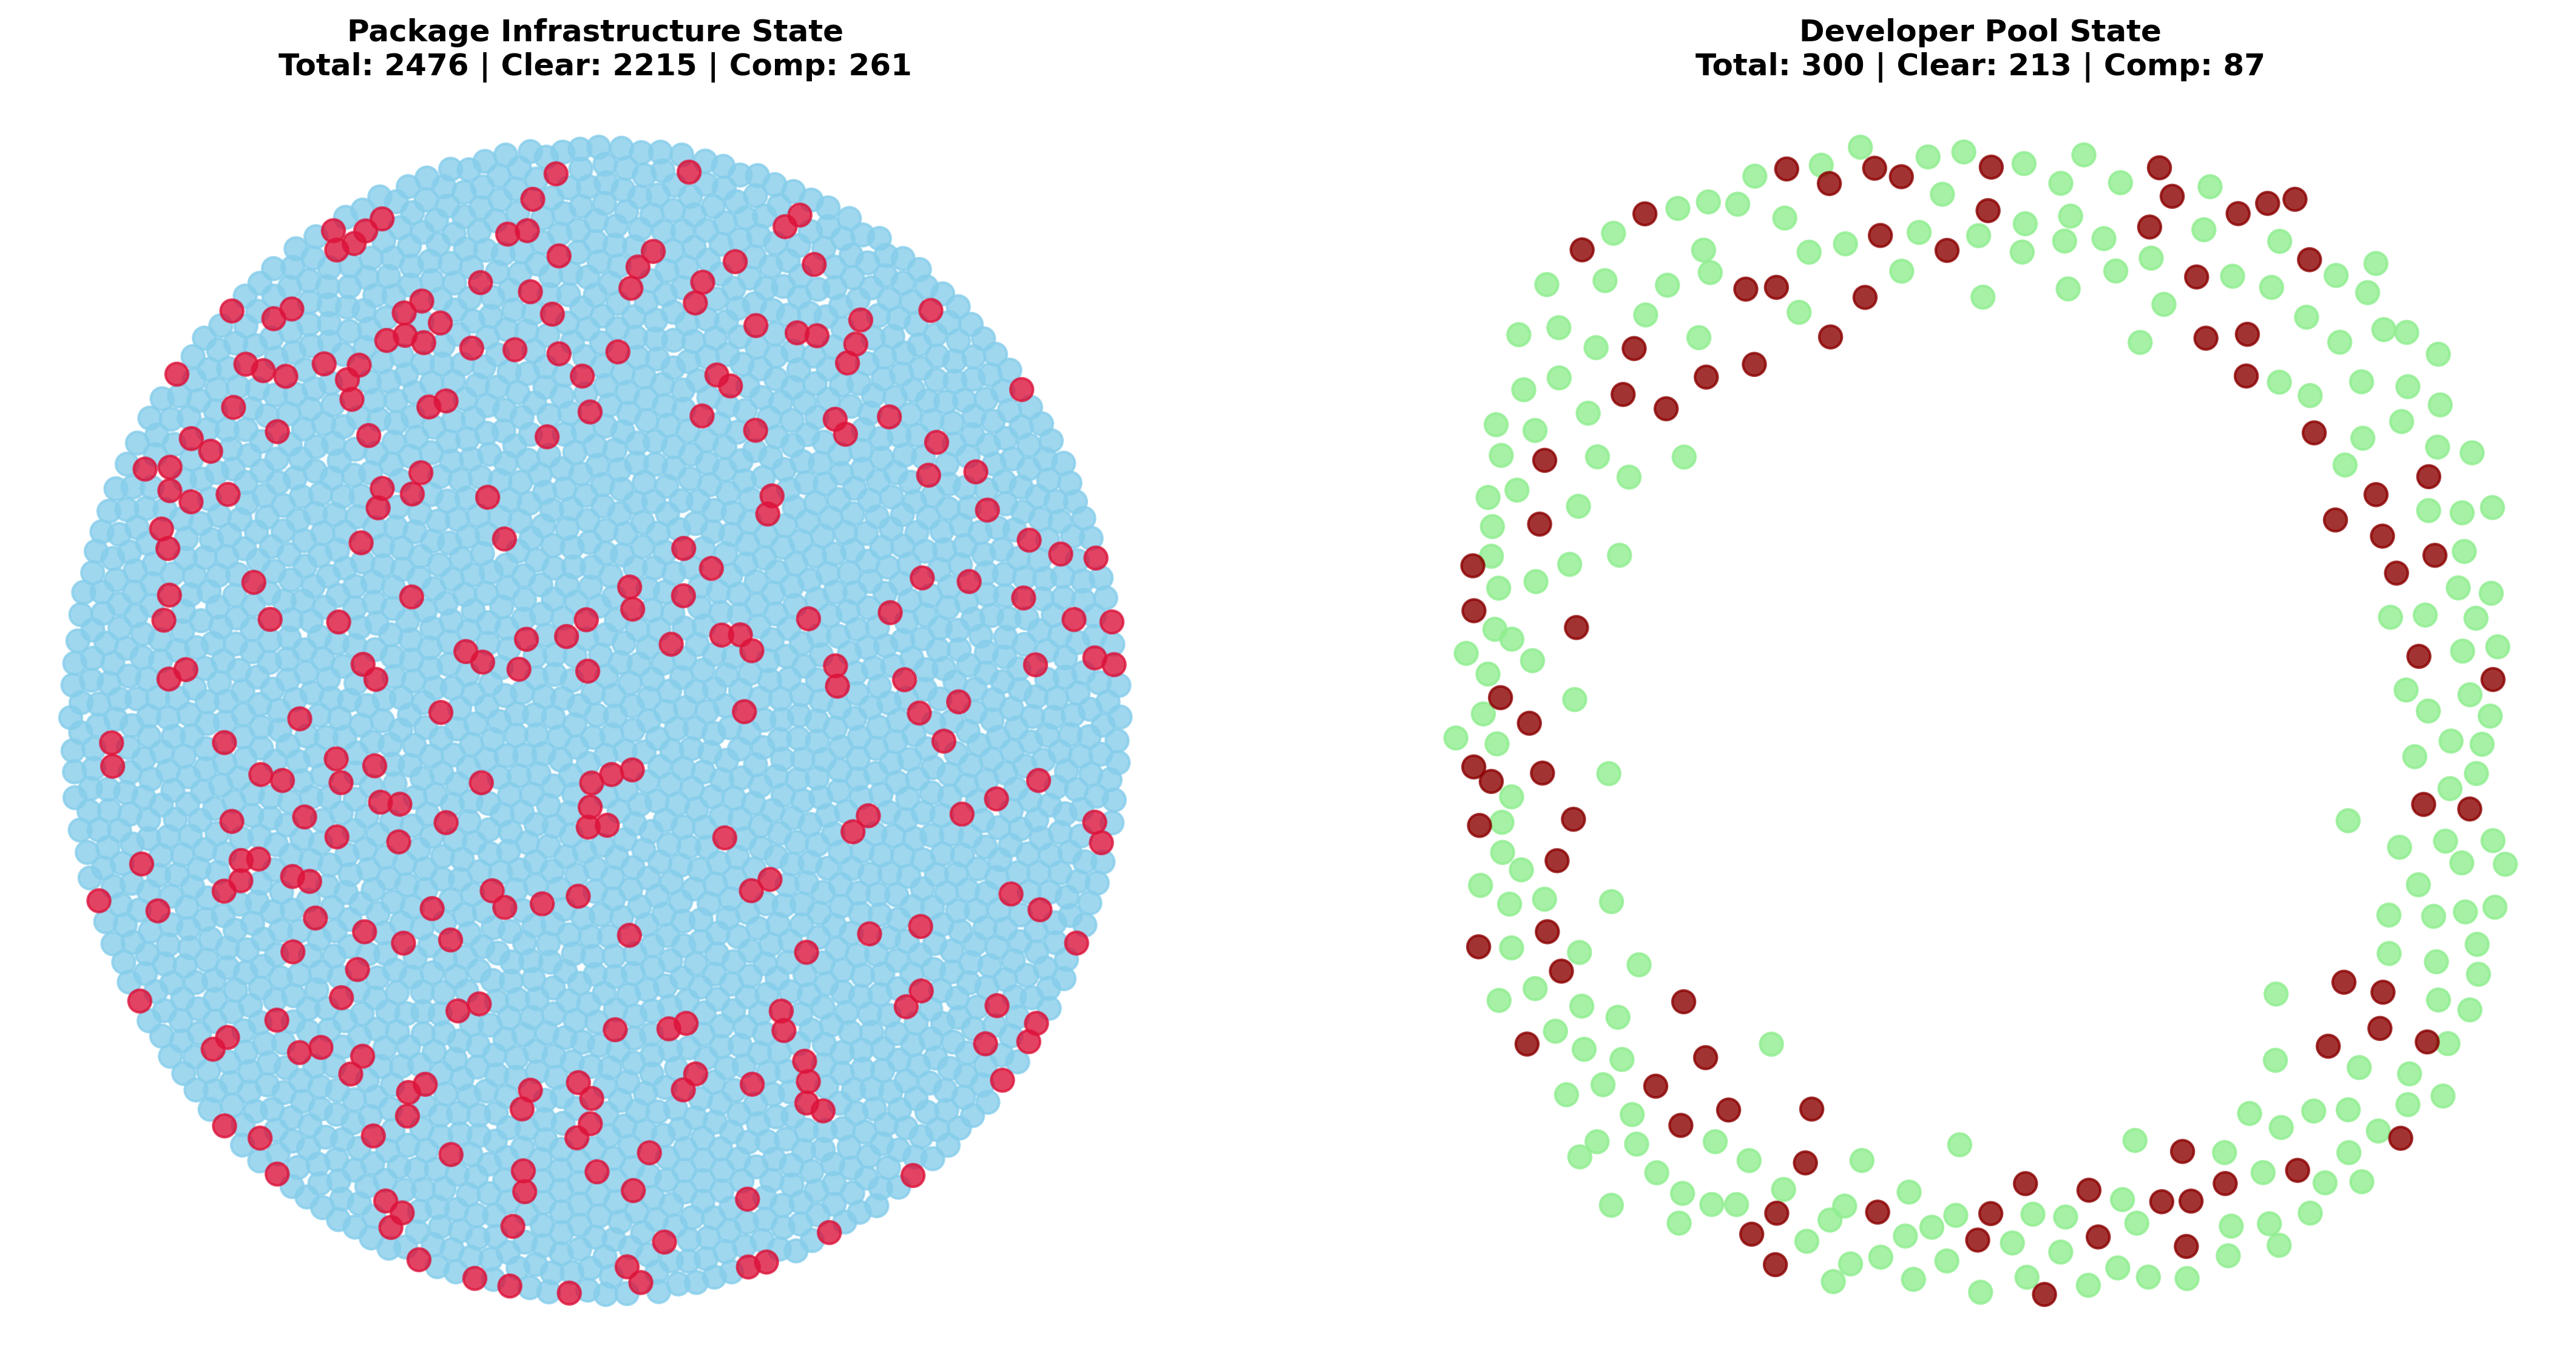
\includegraphics[width=1.0\textwidth]{../figures/integrity_snapshot_in_simulation.png}
    \caption{Integrity snapshot of the simulation.}
    \label{fig:integrity_snapshot_in_simulation}
\end{figure}

However, this simulation is an abstract model designed to represent reality within a limited framework, consisting of an environment, defined rules, entities, specific behaviors, and a temporal structure (using either tick- based steps or event-based sequences). While simulations are essential for predictive analysis in scenarios that are too costly or dangerous to test in the real world, they are inherently prone to "drift". Without continuous recalibration, a model can rapidly diverge from reality, especially when major real-world shifts occur that the simulation cannot account for due to its predefined, static boundaries. Beyond these challenges, our simulation is subject to several other specific assumptions and limitations:
\begin{itemize}
    \item Closed ecosystem environment - the simulation operates as a strictly closed system focused on a single repository without mirrors. Additionally, we assume the platform infrastructure itself is immutable and cannot be compromised.
    \item Stochasticity and randomness - event probabilities and distributions rely on pseudo-random number generation (via the Python standard library random module, which interfaces with /dev/urandom or /dev/random on Linux).
    \item Absence of actor confrontation - the model does not account for direct confrontations or interference between different actors, such as active conflicts between competing threat actors.
    \item Simplified network logistics - network-level variables, such as latency, bandwidth constraints, or connectivity issues during package uploads and downloads, are not represented.
    \item Scaling constraints - the total volume of packages and agents is significantly lower than the scales observed in real-world ecosystems.
    \item Agents have predefined roles, but in reality, they can shift between / act on multiple roles simultaneously. For example, a package publisher can do the same things as a regular user. Moreover, some developers and package publishers can be malicious like regular threat actors, but we assume that they have passively good intensions or behavior with goodwill.
    \item Single-project assumption - each developer or user is limited to one active project at a time. Consequently, all dependencies are grouped into a single pool rather than being isolated by specific projects or environments.
    \item Lack of organizational structure - the simulation does not represent organized groups, teams, or corporate entities. So, it misses the collaborative nature of departments (e.g., data science teams favor specific libraries like “numpy”) and the influence of internal company policies or domain- specific dependency preferences.
    \item Manual vs. automated actions - the model exclusively simulates manual interactions performed by a person via a package manager toolkit. It excludes automated CI/CD pipelines, build scripts, and automated test environments that frequently pull packages from repositories.
    \item Direct dependency focus - the simulation only accounts for direct dependencies. Supply chain attacks via transitive dependencies are excluded, as these would require a full dependency resolution implementation. Some of these trends, specifically regarding how threat actors affect compromised package variation, are illustrated in Figure \ref{fig:attack_grid_on_dependencies}.
\end{itemize}

\begin{figure}[htbp]
    \centering
    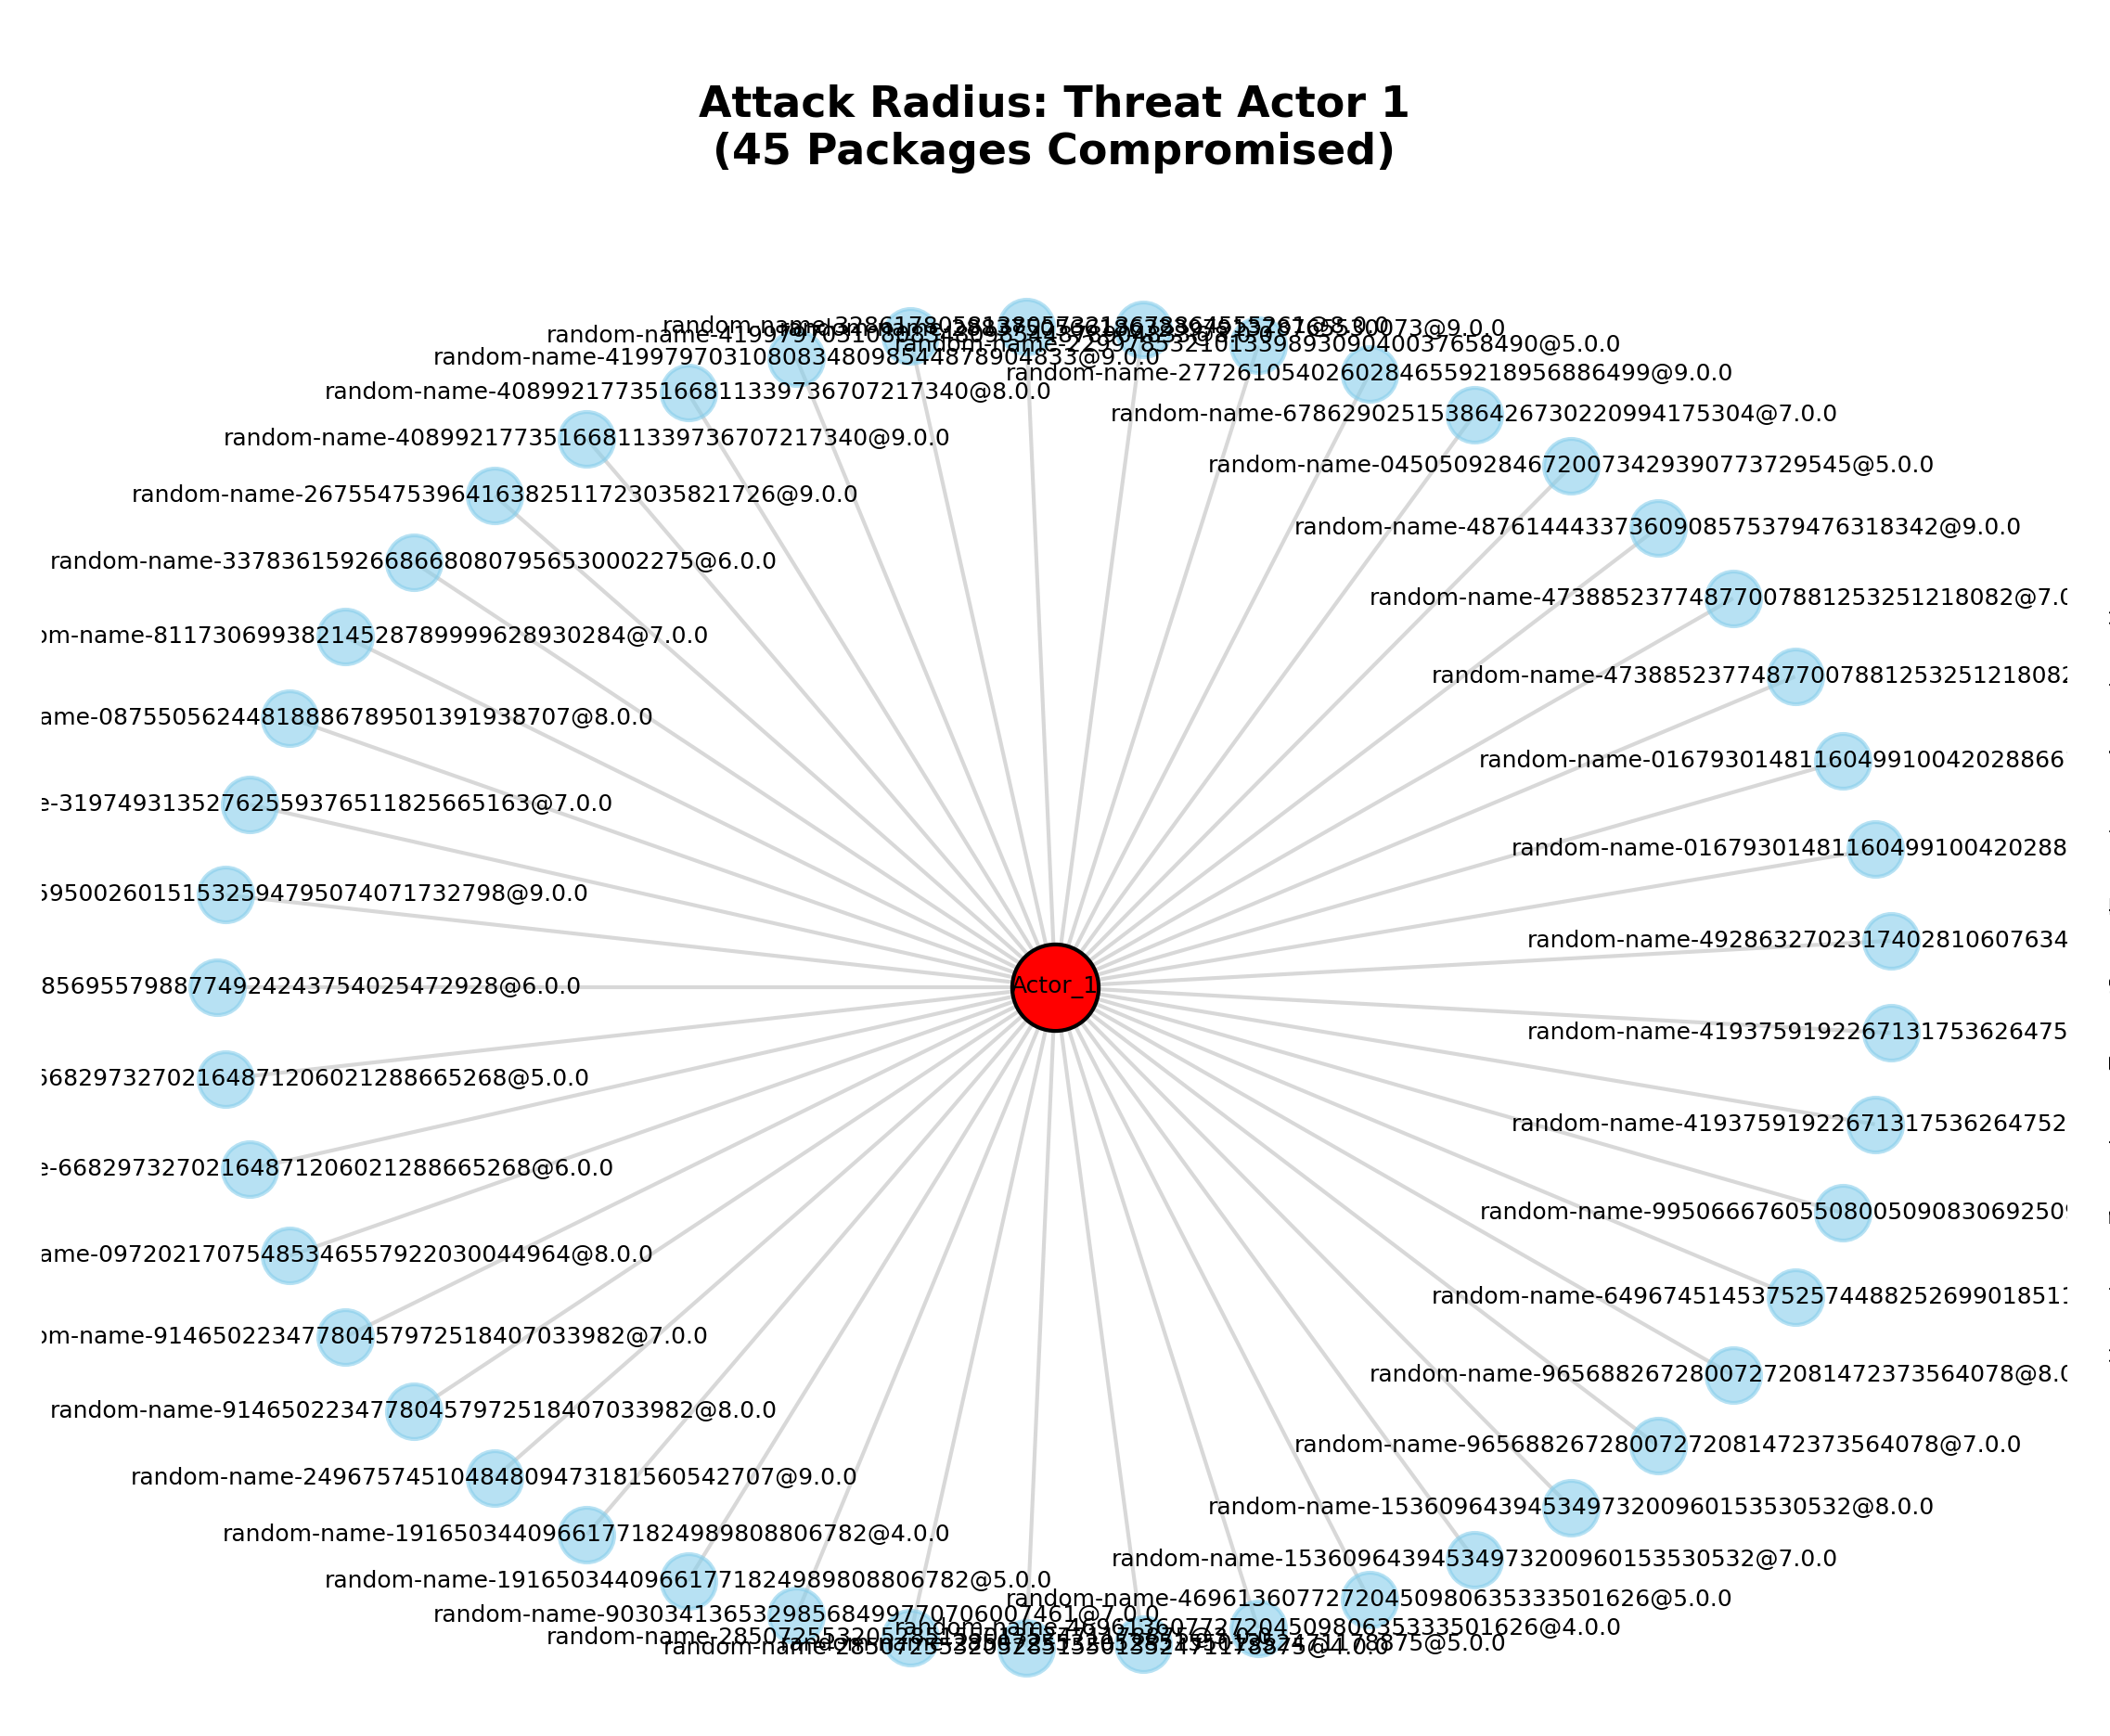
\includegraphics[width=1.0\textwidth]{../figures/attack_grid_on_dependencies.png}
    \caption{Example of single threat actor with a relationship to his produced compromised packages in a simulation iteration.}
    \label{fig:attack_grid_on_dependencies}
\end{figure}

\newpage

By simulating a complex dynamic system across both micro and macro levels, we can analyze how these quality gates and restrictive policies effectively reduce the propagation speed of malware, vulnerabilities, and supply chain attacks. These gates can protect and regulate thecommunity by temporarily blocking packages based on various factors, moving them through lifecycle states such as under consideration, public, blocked, or reported. In this paradigm, both actors and packages carry implicit and explicit trust levels, representing either internal peer opinions or external platform scores, which shift dynamically based on observed compromises. It is important to note that in a real-world environment, neither static nor dynamic preventive scanners are absolute, so preventive measures should be combined with reactive approaches to create a multi-layered defense.

Regarding the platform architecture, we decided to implement the analysis engine components as separate entities to facilitate concurrency and asynchronous inter- process communications across multiple instances to prevent performance bottlenecks. On the other hand, there are still unresolved issues regarding software isolation:
\begin{itemize}
    \item Emulation and virtualization differ from physical hardware in both performance and qualitative properties, often preventing hardware-level vulnerabilities or side-channel attacks from manifesting accurately. Sophisticated software may employ evasion techniques to detect these isolated environments, allowing it to hide malicious behavior or cease execution entirely. Even techniques like hardware rotation or mimicking the characteristics of physical devices often fail, as real hardware continues to behave differently under specific conditions.
    \item The risk of escapes from isolated environments necessitates constant updates to keep the analysis environment secure, requiring ongoing maintenance such as replacing outdated third-party tools, integrating emerging detection techniques, and reconfiguring monitoring systems.
    \item Certain software requires manual intervention that disrupts full automation, such as patching binaries or recompiling source code.
\end{itemize}

\section{Practical analysis of Android-compatible devices for general-purpose computations}
\subsection{Data gathering and descriptions of dataset}

We gathered a dataset from public sources consisting of Android-compatible smartphones ranging from Android version 1 to 16 and beyond, containing 1745 unique models after pre-processing. The primary objective was to study security issues, unique features, and general complexities of utilizing such devices as low-end nodes. Firstly, detailed description of the dataset is provided in Table \ref{tab:android_dataset_description}. Secondly, data collection was carried out manually and through Python scripts. Thirdly, visualizations were rendered in Matplotlib and processed using Pandas, while the raw data was saved in a structured JSON format. Finally, the remaining details are described in more depth in the repository containing our source materials \cite{tendikov2026iccsfai}.

\begin{table}[htbp]
    \centering
    \begin{tabular}{|l|p{10cm}|}
        \hline
        \textbf{Fields} & \textbf{Data type and description} \\
        \hline
        model & str; the formal or consumer name of the device model \\
        \hline
        developer & str; the manufacturer or vendor that developed, sells, or brands the specific device instance \\
        \hline
        release\_date & datetime; the date of public release for consumer purchase \\
        \hline
        android\_version & str; the stock version at release or the default minimal version supported by the smartphone in normalized form (``major.minor.patch'') \\
        \hline
        status & str; one of the possible statuses for the smartphone's Android version (latest, unknown, supported, or unsupported) \\
        \hline
        latest\_security\_patch\_date & datetime; the date of the latest / last security patch released for the smartphone's Android version \\
        \hline
    \end{tabular}
    \caption{Description of dataset with Android smartphones}
    \label{tab:android_dataset_description}
\end{table}

\subsection{Analysis results and statistical charts from the dataset of devices}

Figure \ref{fig:major_version_distribution} represents the major Android versions across the collected dataset of smartphones, where popularity peaks are visible at versions 4, 10, and 11. Unclear decline is also noticeable starting from version 11, but it is most likely related to the limited sample size in our dataset, possible drop in  interest in Android devices, a reduction in smartphone model segments, monopolization around a limited number of manufacturers, or limited support for the latest Android versions from custom distributions (e.g., MIUI, OneUI, etc.). The graph illustrates that there are 980 devices with Android versions ranging from 1 to 9 out of the 1742 shown in total, indicating a massive volume of old or legacy devices that require attention in order to find practical Major Android Versionsaacross Smartphonesuse for them.

\begin{figure}[htbp]
    \centering
    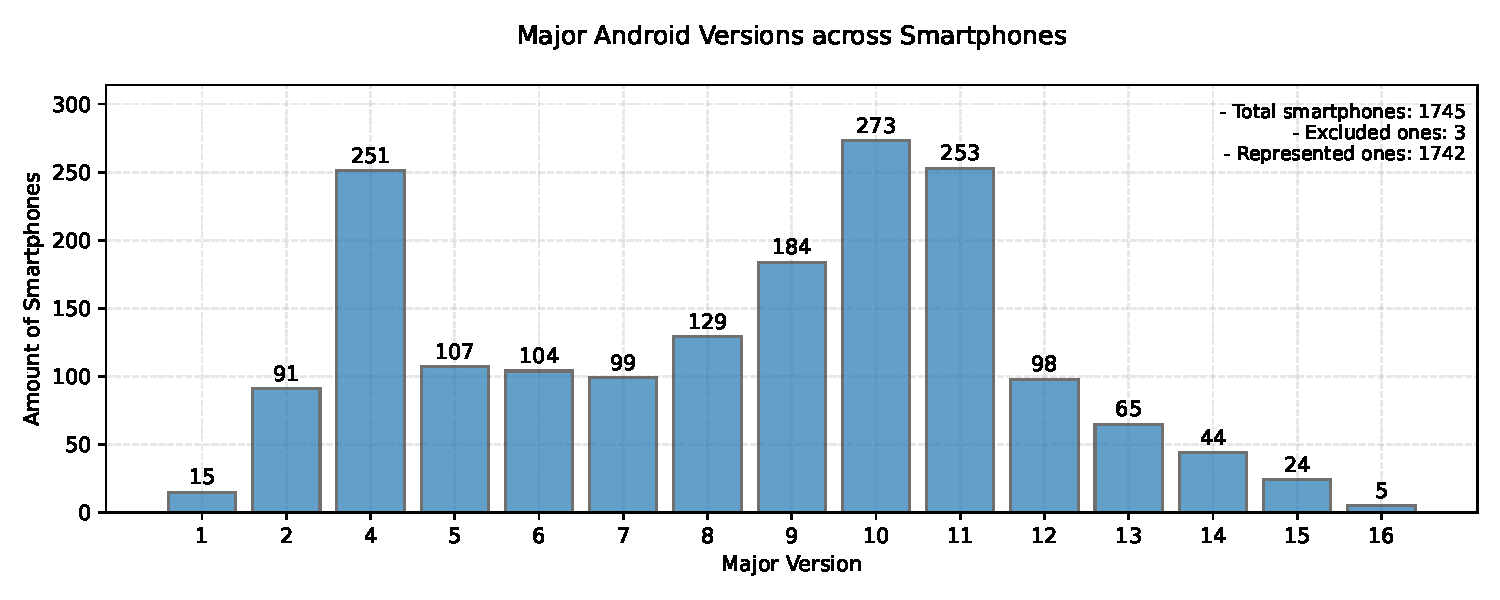
\includegraphics[width=0.6\textwidth]{../figures/major_version_distribution.pdf}
    \caption{Major Android versions across smartphone models, excluding certain smartphones due to inconsistencies in their versioning semantics and unconfirmed / unknown Android versions on them.}
    \label{fig:major_version_distribution}
\end{figure}

Figure \ref{fig:android_3_groups_comparison} groups devices by their versions relative to support for Termux which is a terminal emulator for Android that allows running ported binaries, scripts, or acting similar to Linux distribution environment, rather than creating a separate application with calls to the Android API. Notably, the majority of devices of 67.4\% fall into the compatible category that we are targeting, while the remaining 32.6\% represent a problematic segment that is difficult to work with and maintain.

\begin{figure}[htbp]
    \centering
    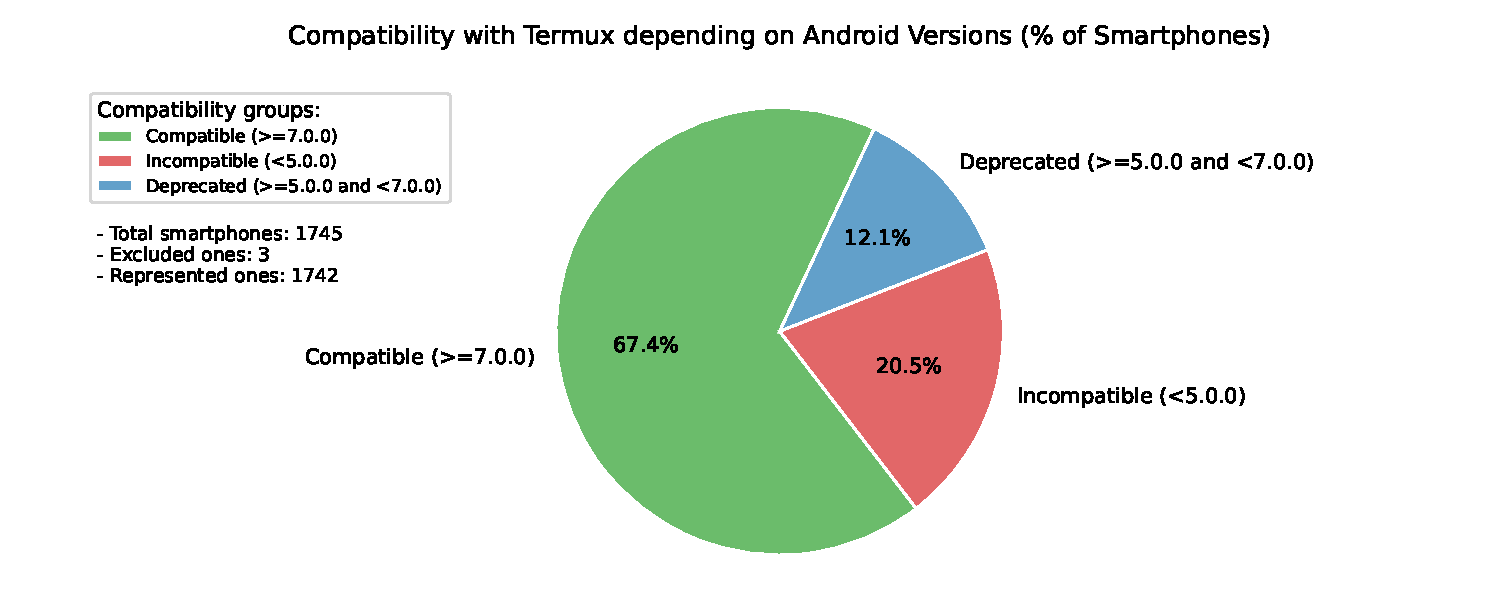
\includegraphics[width=1.0\textwidth]{../figures/android_3_groups_comparison.pdf}
    \caption{Compatibility with Termux depending on Android versions (\% of smartphones). Deprecated status formally means that it works on older versions without the Termux package ecosystem, which requires building packages from source. Other incompatibles might be mitigated by manually porting Termux with wrappers over the Android API for specific old versions, but without proper support or patches for kernel vulnerabilities.}
    \label{fig:android_3_groups_comparison}
\end{figure}

Figure \ref{fig:phone_android_version_status_distribution} and \ref{fig:android_latest_patches_and_smartphones_release_dates} address security and the level of support these devices receive in terms of Android version and kernel updates. The Android version status for 1669 devices is "unsupported", meaning the version is not the latest and has reached end-of-life which is largely applies to all versions except 15 and 16. Of course, this does not rule out the existence of backports from Google when necessary, nor does it exclude support models provided by manufacturers for custom firmware. Figure \ref{fig:android_latest_patches_and_smartphones_release_dates} expands on this understanding by detailing critical facts regarding smartphone releases, with a peak in 2019 and 2020. Furthermore, the security aspect is examined from the perspective of the latest security patch, which reveals that approximately 66.78\%, amounting to 989 out of 1481 devices, received their latest security patches for their Android version three or more years ago.

\begin{figure}[htbp]
    \centering
    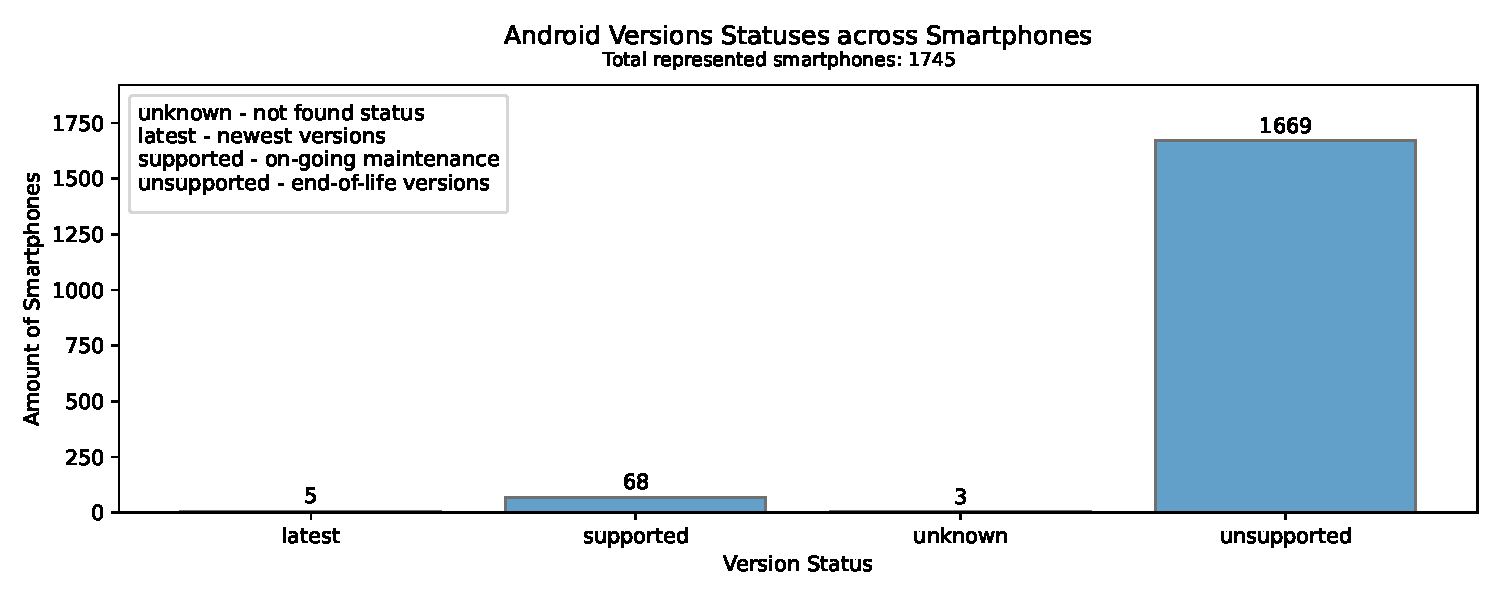
\includegraphics[width=1.0\textwidth]{../figures/phone_android_version_status_distribution.pdf}
    \caption{Device statuses, where some are displayed as "unknown" because the Android versions on them were unidentified.}
    \label{fig:phone_android_version_status_distribution}
\end{figure}

\begin{figure}[htbp]
    \centering
    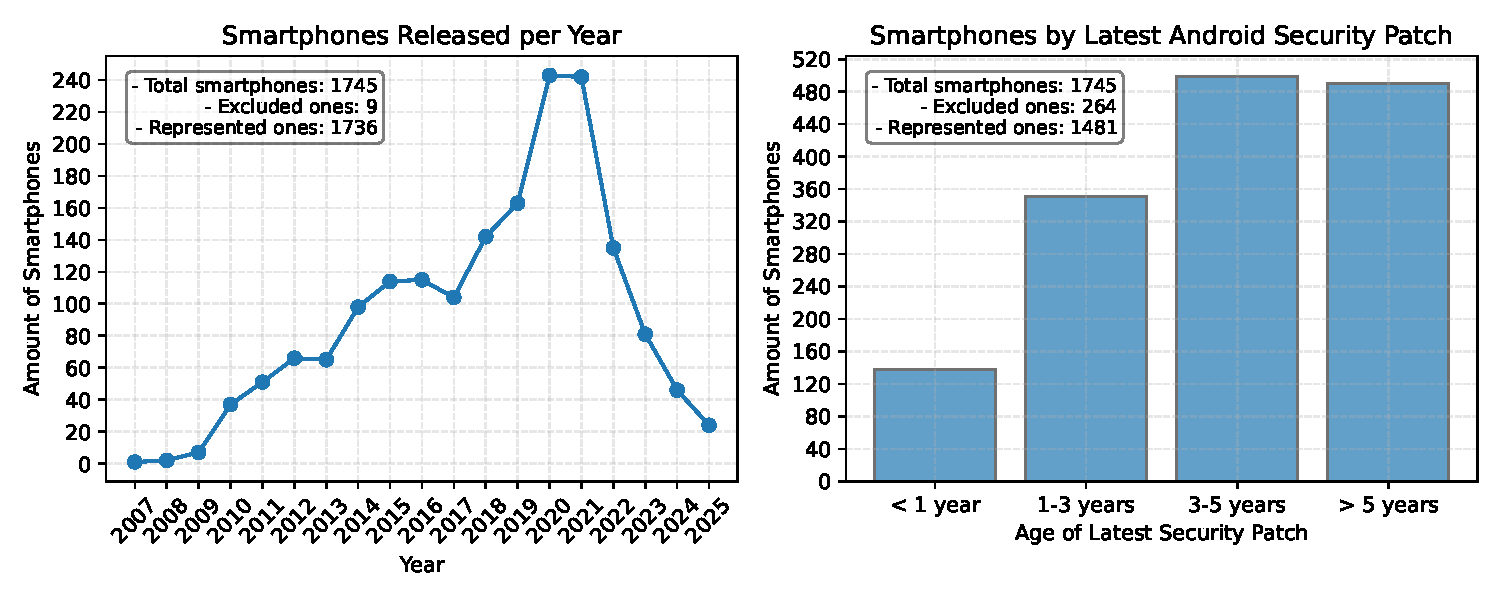
\includegraphics[width=1.0\textwidth]{../figures/android_latest_patches_and_smartphones_release_dates.pdf}
    \caption{Amount of smartphone models released per year and their latest
Android security patches.}
    \label{fig:android_latest_patches_and_smartphones_release_dates}
\end{figure}

\newpage

The utilization of legacy Android smartphones for a distributed network is a complex set of physical and systemic challenges. Because of outdated firmware and unsupported Android versions, these devices are vulnerable to unpatched exploits at both the operating system and kernel levels, requiring significant technical expertise to mitigate through methods such as rooting or installing custom distributions. Consequently, connecting them to the public web poses a substantial security risk. It is only possible to use them in isolated local environments and private networks. Also, these devices struggle to maintain a charge under load for extended periods due to severe battery wear and overall hardware degradation. In some jurisdictions, utilizing such devices is prohibited under European Union energy standards because they are potential fire hazards and are significantly less efficient, resulting in higher power consumption with lower performance output.

The network still faces other unresolved and ambiguous issues. Firstly, the proof-of-burn mechanic may discourage certain participants due to the permanent loss of accumulated wealth. Furthermore, scenarios may arise where the total supply is depleted while existing tokens remain unburned, resulting in a liquidity crisis for new participants due to the limited overall token availability. Our initial intent was to incentivize the constant circulation of capital rather than passive holding, thereby mitigating the influence of large-scale stakeholders over network control. Secondly, we had ideas to explore an investment mechanism involving registered public entities, such as universities or charities. For example, users could delegate tokens to these organizations to defer the burn rate for a specified period. However, it is not sustainable due to potential exploitation schemes, such as the use of cryptocurrency tumblers and mixers to cycle tokens between accounts, or the deployment of empty contracts by bot farms to manipulate network activity. Thirdly, social and trust factors remain unavoidable, as actors may intentionally or unintentionally engage in activities such as providing low-quality results (empty data labels, fake model inference, incompleted submissions, and different disruptions by repeating actions as a form of distributed denial-of-service attack), organizing collusions, and other malicious schemes. So, the network may need external validators for quality assessment and moderation, as well as collaboration with local government authorities to implement user verification through the proof-of-identity and the enforcement of more restrictive operational limits.
